
% Default to the notebook output style

    


% Inherit from the specified cell style.




    
\documentclass{article}

    
    
    \usepackage{graphicx} % Used to insert images
    \usepackage{adjustbox} % Used to constrain images to a maximum size 
    \usepackage{color} % Allow colors to be defined
    \usepackage{enumerate} % Needed for markdown enumerations to work
    \usepackage{geometry} % Used to adjust the document margins
    \usepackage{amsmath} % Equations
    \usepackage{amssymb} % Equations
    \usepackage{eurosym} % defines \euro
    \usepackage[mathletters]{ucs} % Extended unicode (utf-8) support
    \usepackage[utf8x]{inputenc} % Allow utf-8 characters in the tex document
    \usepackage{fancyvrb} % verbatim replacement that allows latex
    \usepackage{grffile} % extends the file name processing of package graphics 
                         % to support a larger range 
    % The hyperref package gives us a pdf with properly built
    % internal navigation ('pdf bookmarks' for the table of contents,
    % internal cross-reference links, web links for URLs, etc.)
    \usepackage{hyperref}
    \usepackage{longtable} % longtable support required by pandoc >1.10
    \usepackage{booktabs}  % table support for pandoc > 1.12.2
    \usepackage{indentfirst}

    
    
    \definecolor{orange}{cmyk}{0,0.4,0.8,0.2}
    \definecolor{darkorange}{rgb}{.71,0.21,0.01}
    \definecolor{darkgreen}{rgb}{.12,.54,.11}
    \definecolor{myteal}{rgb}{.26, .44, .56}
    \definecolor{gray}{gray}{0.45}
    \definecolor{lightgray}{gray}{.95}
    \definecolor{mediumgray}{gray}{.8}
    \definecolor{inputbackground}{rgb}{.95, .95, .85}
    \definecolor{outputbackground}{rgb}{.95, .95, .95}
    \definecolor{traceback}{rgb}{1, .95, .95}
    % ansi colors
    \definecolor{red}{rgb}{.6,0,0}
    \definecolor{green}{rgb}{0,.65,0}
    \definecolor{brown}{rgb}{0.6,0.6,0}
    \definecolor{blue}{rgb}{0,.145,.698}
    \definecolor{purple}{rgb}{.698,.145,.698}
    \definecolor{cyan}{rgb}{0,.698,.698}
    \definecolor{lightgray}{gray}{0.5}
    
    % bright ansi colors
    \definecolor{darkgray}{gray}{0.25}
    \definecolor{lightred}{rgb}{1.0,0.39,0.28}
    \definecolor{lightgreen}{rgb}{0.48,0.99,0.0}
    \definecolor{lightblue}{rgb}{0.53,0.81,0.92}
    \definecolor{lightpurple}{rgb}{0.87,0.63,0.87}
    \definecolor{lightcyan}{rgb}{0.5,1.0,0.83}
    
    % commands and environments needed by pandoc snippets
    % extracted from the output of `pandoc -s`
    \providecommand{\tightlist}{%
      \setlength{\itemsep}{0pt}\setlength{\parskip}{0pt}}
    \DefineVerbatimEnvironment{Highlighting}{Verbatim}{commandchars=\\\{\}}
    % Add ',fontsize=\small' for more characters per line
    \newenvironment{Shaded}{}{}
    \newcommand{\KeywordTok}[1]{\textcolor[rgb]{0.00,0.44,0.13}{\textbf{{#1}}}}
    \newcommand{\DataTypeTok}[1]{\textcolor[rgb]{0.56,0.13,0.00}{{#1}}}
    \newcommand{\DecValTok}[1]{\textcolor[rgb]{0.25,0.63,0.44}{{#1}}}
    \newcommand{\BaseNTok}[1]{\textcolor[rgb]{0.25,0.63,0.44}{{#1}}}
    \newcommand{\FloatTok}[1]{\textcolor[rgb]{0.25,0.63,0.44}{{#1}}}
    \newcommand{\CharTok}[1]{\textcolor[rgb]{0.25,0.44,0.63}{{#1}}}
    \newcommand{\StringTok}[1]{\textcolor[rgb]{0.25,0.44,0.63}{{#1}}}
    \newcommand{\CommentTok}[1]{\textcolor[rgb]{0.38,0.63,0.69}{\textit{{#1}}}}
    \newcommand{\OtherTok}[1]{\textcolor[rgb]{0.00,0.44,0.13}{{#1}}}
    \newcommand{\AlertTok}[1]{\textcolor[rgb]{1.00,0.00,0.00}{\textbf{{#1}}}}
    \newcommand{\FunctionTok}[1]{\textcolor[rgb]{0.02,0.16,0.49}{{#1}}}
    \newcommand{\RegionMarkerTok}[1]{{#1}}
    \newcommand{\ErrorTok}[1]{\textcolor[rgb]{1.00,0.00,0.00}{\textbf{{#1}}}}
    \newcommand{\NormalTok}[1]{{#1}}
    
    % Define a nice break command that doesn't care if a line doesn't already
    % exist.
    \def\br{\hspace*{\fill} \\* }
    % Math Jax compatability definitions
    \def\gt{>}
    \def\lt{<}
    % Document parameters
    \title{Homework 3}
    \author{Roly Vicar\'ia \\ STAT501 Fall 2015}   
    
    

    % Pygments definitions
    
\makeatletter
\def\PY@reset{\let\PY@it=\relax \let\PY@bf=\relax%
    \let\PY@ul=\relax \let\PY@tc=\relax%
    \let\PY@bc=\relax \let\PY@ff=\relax}
\def\PY@tok#1{\csname PY@tok@#1\endcsname}
\def\PY@toks#1+{\ifx\relax#1\empty\else%
    \PY@tok{#1}\expandafter\PY@toks\fi}
\def\PY@do#1{\PY@bc{\PY@tc{\PY@ul{%
    \PY@it{\PY@bf{\PY@ff{#1}}}}}}}
\def\PY#1#2{\PY@reset\PY@toks#1+\relax+\PY@do{#2}}

\expandafter\def\csname PY@tok@gd\endcsname{\def\PY@tc##1{\textcolor[rgb]{0.63,0.00,0.00}{##1}}}
\expandafter\def\csname PY@tok@gu\endcsname{\let\PY@bf=\textbf\def\PY@tc##1{\textcolor[rgb]{0.50,0.00,0.50}{##1}}}
\expandafter\def\csname PY@tok@gt\endcsname{\def\PY@tc##1{\textcolor[rgb]{0.00,0.27,0.87}{##1}}}
\expandafter\def\csname PY@tok@gs\endcsname{\let\PY@bf=\textbf}
\expandafter\def\csname PY@tok@gr\endcsname{\def\PY@tc##1{\textcolor[rgb]{1.00,0.00,0.00}{##1}}}
\expandafter\def\csname PY@tok@cm\endcsname{\let\PY@it=\textit\def\PY@tc##1{\textcolor[rgb]{0.25,0.50,0.50}{##1}}}
\expandafter\def\csname PY@tok@vg\endcsname{\def\PY@tc##1{\textcolor[rgb]{0.10,0.09,0.49}{##1}}}
\expandafter\def\csname PY@tok@m\endcsname{\def\PY@tc##1{\textcolor[rgb]{0.40,0.40,0.40}{##1}}}
\expandafter\def\csname PY@tok@mh\endcsname{\def\PY@tc##1{\textcolor[rgb]{0.40,0.40,0.40}{##1}}}
\expandafter\def\csname PY@tok@go\endcsname{\def\PY@tc##1{\textcolor[rgb]{0.53,0.53,0.53}{##1}}}
\expandafter\def\csname PY@tok@ge\endcsname{\let\PY@it=\textit}
\expandafter\def\csname PY@tok@vc\endcsname{\def\PY@tc##1{\textcolor[rgb]{0.10,0.09,0.49}{##1}}}
\expandafter\def\csname PY@tok@il\endcsname{\def\PY@tc##1{\textcolor[rgb]{0.40,0.40,0.40}{##1}}}
\expandafter\def\csname PY@tok@cs\endcsname{\let\PY@it=\textit\def\PY@tc##1{\textcolor[rgb]{0.25,0.50,0.50}{##1}}}
\expandafter\def\csname PY@tok@cp\endcsname{\def\PY@tc##1{\textcolor[rgb]{0.74,0.48,0.00}{##1}}}
\expandafter\def\csname PY@tok@gi\endcsname{\def\PY@tc##1{\textcolor[rgb]{0.00,0.63,0.00}{##1}}}
\expandafter\def\csname PY@tok@gh\endcsname{\let\PY@bf=\textbf\def\PY@tc##1{\textcolor[rgb]{0.00,0.00,0.50}{##1}}}
\expandafter\def\csname PY@tok@ni\endcsname{\let\PY@bf=\textbf\def\PY@tc##1{\textcolor[rgb]{0.60,0.60,0.60}{##1}}}
\expandafter\def\csname PY@tok@nl\endcsname{\def\PY@tc##1{\textcolor[rgb]{0.63,0.63,0.00}{##1}}}
\expandafter\def\csname PY@tok@nn\endcsname{\let\PY@bf=\textbf\def\PY@tc##1{\textcolor[rgb]{0.00,0.00,1.00}{##1}}}
\expandafter\def\csname PY@tok@no\endcsname{\def\PY@tc##1{\textcolor[rgb]{0.53,0.00,0.00}{##1}}}
\expandafter\def\csname PY@tok@na\endcsname{\def\PY@tc##1{\textcolor[rgb]{0.49,0.56,0.16}{##1}}}
\expandafter\def\csname PY@tok@nb\endcsname{\def\PY@tc##1{\textcolor[rgb]{0.00,0.50,0.00}{##1}}}
\expandafter\def\csname PY@tok@nc\endcsname{\let\PY@bf=\textbf\def\PY@tc##1{\textcolor[rgb]{0.00,0.00,1.00}{##1}}}
\expandafter\def\csname PY@tok@nd\endcsname{\def\PY@tc##1{\textcolor[rgb]{0.67,0.13,1.00}{##1}}}
\expandafter\def\csname PY@tok@ne\endcsname{\let\PY@bf=\textbf\def\PY@tc##1{\textcolor[rgb]{0.82,0.25,0.23}{##1}}}
\expandafter\def\csname PY@tok@nf\endcsname{\def\PY@tc##1{\textcolor[rgb]{0.00,0.00,1.00}{##1}}}
\expandafter\def\csname PY@tok@si\endcsname{\let\PY@bf=\textbf\def\PY@tc##1{\textcolor[rgb]{0.73,0.40,0.53}{##1}}}
\expandafter\def\csname PY@tok@s2\endcsname{\def\PY@tc##1{\textcolor[rgb]{0.73,0.13,0.13}{##1}}}
\expandafter\def\csname PY@tok@vi\endcsname{\def\PY@tc##1{\textcolor[rgb]{0.10,0.09,0.49}{##1}}}
\expandafter\def\csname PY@tok@nt\endcsname{\let\PY@bf=\textbf\def\PY@tc##1{\textcolor[rgb]{0.00,0.50,0.00}{##1}}}
\expandafter\def\csname PY@tok@nv\endcsname{\def\PY@tc##1{\textcolor[rgb]{0.10,0.09,0.49}{##1}}}
\expandafter\def\csname PY@tok@s1\endcsname{\def\PY@tc##1{\textcolor[rgb]{0.73,0.13,0.13}{##1}}}
\expandafter\def\csname PY@tok@kd\endcsname{\let\PY@bf=\textbf\def\PY@tc##1{\textcolor[rgb]{0.00,0.50,0.00}{##1}}}
\expandafter\def\csname PY@tok@sh\endcsname{\def\PY@tc##1{\textcolor[rgb]{0.73,0.13,0.13}{##1}}}
\expandafter\def\csname PY@tok@sc\endcsname{\def\PY@tc##1{\textcolor[rgb]{0.73,0.13,0.13}{##1}}}
\expandafter\def\csname PY@tok@sx\endcsname{\def\PY@tc##1{\textcolor[rgb]{0.00,0.50,0.00}{##1}}}
\expandafter\def\csname PY@tok@bp\endcsname{\def\PY@tc##1{\textcolor[rgb]{0.00,0.50,0.00}{##1}}}
\expandafter\def\csname PY@tok@c1\endcsname{\let\PY@it=\textit\def\PY@tc##1{\textcolor[rgb]{0.25,0.50,0.50}{##1}}}
\expandafter\def\csname PY@tok@kc\endcsname{\let\PY@bf=\textbf\def\PY@tc##1{\textcolor[rgb]{0.00,0.50,0.00}{##1}}}
\expandafter\def\csname PY@tok@c\endcsname{\let\PY@it=\textit\def\PY@tc##1{\textcolor[rgb]{0.25,0.50,0.50}{##1}}}
\expandafter\def\csname PY@tok@mf\endcsname{\def\PY@tc##1{\textcolor[rgb]{0.40,0.40,0.40}{##1}}}
\expandafter\def\csname PY@tok@err\endcsname{\def\PY@bc##1{\setlength{\fboxsep}{0pt}\fcolorbox[rgb]{1.00,0.00,0.00}{1,1,1}{\strut ##1}}}
\expandafter\def\csname PY@tok@mb\endcsname{\def\PY@tc##1{\textcolor[rgb]{0.40,0.40,0.40}{##1}}}
\expandafter\def\csname PY@tok@ss\endcsname{\def\PY@tc##1{\textcolor[rgb]{0.10,0.09,0.49}{##1}}}
\expandafter\def\csname PY@tok@sr\endcsname{\def\PY@tc##1{\textcolor[rgb]{0.73,0.40,0.53}{##1}}}
\expandafter\def\csname PY@tok@mo\endcsname{\def\PY@tc##1{\textcolor[rgb]{0.40,0.40,0.40}{##1}}}
\expandafter\def\csname PY@tok@kn\endcsname{\let\PY@bf=\textbf\def\PY@tc##1{\textcolor[rgb]{0.00,0.50,0.00}{##1}}}
\expandafter\def\csname PY@tok@mi\endcsname{\def\PY@tc##1{\textcolor[rgb]{0.40,0.40,0.40}{##1}}}
\expandafter\def\csname PY@tok@gp\endcsname{\let\PY@bf=\textbf\def\PY@tc##1{\textcolor[rgb]{0.00,0.00,0.50}{##1}}}
\expandafter\def\csname PY@tok@o\endcsname{\def\PY@tc##1{\textcolor[rgb]{0.40,0.40,0.40}{##1}}}
\expandafter\def\csname PY@tok@kr\endcsname{\let\PY@bf=\textbf\def\PY@tc##1{\textcolor[rgb]{0.00,0.50,0.00}{##1}}}
\expandafter\def\csname PY@tok@s\endcsname{\def\PY@tc##1{\textcolor[rgb]{0.73,0.13,0.13}{##1}}}
\expandafter\def\csname PY@tok@kp\endcsname{\def\PY@tc##1{\textcolor[rgb]{0.00,0.50,0.00}{##1}}}
\expandafter\def\csname PY@tok@w\endcsname{\def\PY@tc##1{\textcolor[rgb]{0.73,0.73,0.73}{##1}}}
\expandafter\def\csname PY@tok@kt\endcsname{\def\PY@tc##1{\textcolor[rgb]{0.69,0.00,0.25}{##1}}}
\expandafter\def\csname PY@tok@ow\endcsname{\let\PY@bf=\textbf\def\PY@tc##1{\textcolor[rgb]{0.67,0.13,1.00}{##1}}}
\expandafter\def\csname PY@tok@sb\endcsname{\def\PY@tc##1{\textcolor[rgb]{0.73,0.13,0.13}{##1}}}
\expandafter\def\csname PY@tok@k\endcsname{\let\PY@bf=\textbf\def\PY@tc##1{\textcolor[rgb]{0.00,0.50,0.00}{##1}}}
\expandafter\def\csname PY@tok@se\endcsname{\let\PY@bf=\textbf\def\PY@tc##1{\textcolor[rgb]{0.73,0.40,0.13}{##1}}}
\expandafter\def\csname PY@tok@sd\endcsname{\let\PY@it=\textit\def\PY@tc##1{\textcolor[rgb]{0.73,0.13,0.13}{##1}}}

\def\PYZbs{\char`\\}
\def\PYZus{\char`\_}
\def\PYZob{\char`\{}
\def\PYZcb{\char`\}}
\def\PYZca{\char`\^}
\def\PYZam{\char`\&}
\def\PYZlt{\char`\<}
\def\PYZgt{\char`\>}
\def\PYZsh{\char`\#}
\def\PYZpc{\char`\%}
\def\PYZdl{\char`\$}
\def\PYZhy{\char`\-}
\def\PYZsq{\char`\'}
\def\PYZdq{\char`\"}
\def\PYZti{\char`\~}
% for compatibility with earlier versions
\def\PYZat{@}
\def\PYZlb{[}
\def\PYZrb{]}
\makeatother


    % Exact colors from NB
    \definecolor{incolor}{rgb}{0.0, 0.0, 0.5}
    \definecolor{outcolor}{rgb}{0.545, 0.0, 0.0}



    
    % Prevent overflowing lines due to hard-to-break entities
    \sloppy 
    % Setup hyperref package
    \hypersetup{
      breaklinks=true,  % so long urls are correctly broken across lines
      colorlinks=true,
      urlcolor=blue,
      linkcolor=darkorange,
      citecolor=darkgreen,
      }
    % Slightly bigger margins than the latex defaults
    
    \geometry{verbose,tmargin=1in,bmargin=1in,lmargin=1in,rmargin=1in}
    
    

    \begin{document}
    
    
    \maketitle
    
    

    
    \subsubsection{Question 1}\label{question-1}

\begin{enumerate}
\def\labelenumi{\alph{enumi}.}
\tightlist
\item
  Based on the scatterplot, I would expect less uncertainty for homes
  with lower sale prices because I see a lot more data points for lower
  sale prices than there are for homes with higher sale prices. And not
  only are there more data points for lower sale prices, but the points
  are a lot more dense (i.e., closer in y value), whereas the data
  points for higher sale price homes are more scattered.
\end{enumerate}

\begin{figure}[h!]
 \centering
 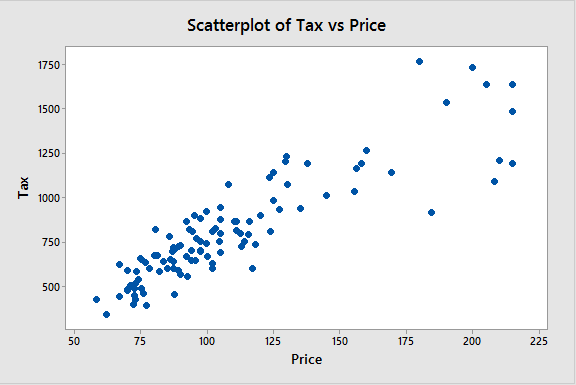
\includegraphics[scale=.5]{./images/scatterplot_tax-vs-price.png}
 % scatterplot_tax-vs-price.png: 576x385 pixel, 96dpi, 15.24x10.19 cm, bb=0 0 432 289
\end{figure}


\begin{enumerate}
\def\labelenumi{\alph{enumi}.}
\setcounter{enumi}{1}
\tightlist
\item
  \(Tax = 61.3 + 6.876 Price\)
\end{enumerate}

\begin{longtable}[c]{@{}lll@{}}
\toprule
Price & 95\% Prediction Interval & Interval Width\tabularnewline
\midrule
\endhead
100 & (466.019, 1031.79) & 565.771\tabularnewline
150 & (808.331, 1377.11) & 568.779\tabularnewline
200 & (1146.12, 1726.96) & 580.84\tabularnewline
\bottomrule
\end{longtable}

\begin{enumerate}
\def\labelenumi{\alph{enumi}.}
\setcounter{enumi}{2}
\tightlist
\item
  \(logTax = 2.076 + 0.9830 logPrice\)
\end{enumerate}

\begin{longtable}[c]{@{}lll@{}}
\toprule
logPrice & 95\% Prediction Interval & Interval Width\tabularnewline
\midrule
\endhead
4.605 & (534.323, 1017.852) & 483.529\tabularnewline
5.011 & (794.657, 1520.463) & 725.806\tabularnewline
5.298 & (1048.777, 2025.456) & 976.679\tabularnewline
\bottomrule
\end{longtable}

\begin{enumerate}
\def\labelenumi{\alph{enumi}.}
\setcounter{enumi}{3}
\tightlist
\item
  The results from parts (b) and (c) confirm my answer from part (a)
  because as the prices (and logPrices) increased, the width of the
  prediction intervals increased also.
\end{enumerate}

    \subsubsection{Question 2}\label{question-2}

\begin{enumerate}
\def\labelenumi{\alph{enumi}.}
\item
  The Lack-of-Fit test for the corn yield indicates that there is a lack
  of linear fit for the model. Without knowing more about the model
  and/or data, I would be hesitant to use this confidence interval.
\item
  In addition to the above, the usefulness of this confidence interval
  is questionable based solely on the fact that the fertizer level is
  outside of the range of observed levels in the dataset.
\item
  This prediction interval is OK to use since the error distribution
  appears close to normal and it seems to meet all the other LINE
  criteria + the fertilizer level is within the scope of the model.
\item
  This prediction interval is NOT OK to use since the error distributino
  does not appear normal and the prediction interval is strongly
  dependent on that.
\item
  This confidence interval is OK to use since the sample size is large
  enough so that the error distribution isn't an issue. And it satisfies
  the other LINE criteria.
\end{enumerate}

    \subsubsection{Question 3}\label{question-3}

\begin{enumerate}
\def\labelenumi{\alph{enumi}.}
\tightlist
\item
  \(Distance = 576.7 - 3.007 Age\)
\end{enumerate}

\begin{figure}[h!]
 \centering
 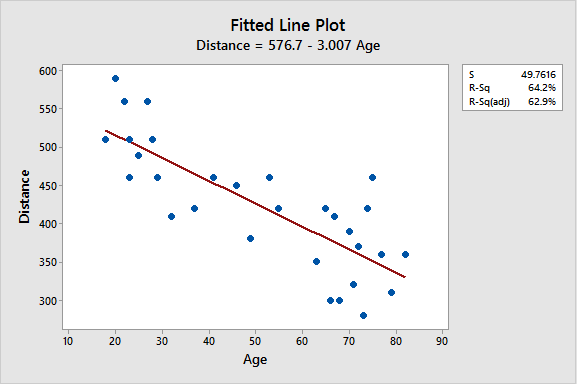
\includegraphics[scale=.5]{./images/scatterplot+regression_distance-vs-age.png}
 % scatterplot+regression_distance-vs-age.png: 577x384 pixel, 96dpi, 15.26x10.16 cm, bb=0 0 433 288
\end{figure}


\begin{enumerate}
\def\labelenumi{\alph{enumi}.}
\setcounter{enumi}{1}
\item
  The slope of the regression line is -3.007. This can be interpreted as
  saying that for every additional year a driver gets older, they see
  about 3 ft less.
\item
  Confidence interval and prediction interval for 75 yrs old
\end{enumerate}

\begin{longtable}[c]{@{}lll@{}}
\toprule
Age & 95\% Confidence Interval & 95\% Prediction Interval\tabularnewline
\midrule
\endhead
75 & (323.213, 379.125) & (245.473, 456.865)\tabularnewline
\bottomrule
\end{longtable}

\begin{enumerate}
\def\labelenumi{\alph{enumi}.}
\setcounter{enumi}{3}
\item
  The ``Fit'' value is calculated by inserting 75 into the regression
  equation: \(576.7 - 3.007(75) \approx 351.175\)
\item
  The confidence interval can be interpreted as saying that we can be
  95\% confident that the mean distance seen by all people age 75 is
  between 323.213 and 379.125 ft.
\item
  The prediction interval can be interpreted as saying that for a random
  75 yr old person, we can be 95\% confident that the distance they can
  see will be between 245.473 and 456.865 ft.
\item
  The fact that the intercept value of this fitted regression is not
  meaningful, does not invalidate the fitted straight line. It just
  means that Age = 0 does not fall within the scope of this model. The
  data used for this model was ages between 18 and 82. We can't really
  trust the regression equation for values outside those ages.
\end{enumerate}

    \subsubsection{Question 4}\label{question-4}

Confidence interval formula:
\(\hat{y}_h \pm t_{(\alpha/2,n-2)} \times \sqrt{MSE \times \left(\frac{1}{n} + \frac{(x_h - \bar{x})^2}{\sum (x_i - \bar{x})^2}\right)}\)

Prediction interval formula:
\(\hat{y}_h \pm t_{(\alpha/2,n-2)} \times \sqrt{MSE \times \left(1 + \frac{1}{n} + \frac{(x_h - \bar{x})^2}{\sum (x_i - \bar{x})^2}\right)}\)

\begin{enumerate}
\def\labelenumi{\alph{enumi}.}
\item
  True. We can see in the formula above, that the second term inside the
  square root becomes zero when \(x_h = \bar{x}\)
\item
  True. The prediction interval formula has an extra MSE term that the
  confidence interval formula does not, so it will always necessarily be
  wider.
\item
  True. If you compute the confidence interval for \(E(Y_h)\) with
  \(X_h = 0\), it would be equal to the confidence interval formula for
  \(\beta_0\), since \(\hat{Y}_h\) would be equal to \(b_0\) and
  \(s(b_0) = s(\hat{Y}_h)\) when \(X_h = 0\).
\item
  True. Since the last term in the prediction interval formula squares
  the difference between \(x_h\) and \(\bar{x}\), it would come out to
  the same value for predictor values equidistant from the sample mean.
\end{enumerate}

    \subsubsection{Question 5}\label{question-5}

\begin{enumerate}
\def\labelenumi{\alph{enumi}.}
\item
  The 95\% confidence interval when Stay = 10 days is: (4.25921,
  4.79849). This interval can be interpreted as saying that we can be
  95\% confident that the infection risk for patients staying in
  hospitals with an average length of stay of 10 days is between 4.259
  and 4.798 percent.
\item
  The 95\% prediction interval when Stay = 10 days is: (2.45891,
  6.59878). This interval can be interpreted as saying that we can be
  95\% confident that the infection risk for patients at a random
  hospital with average stay of 10 days (Mercy Hospital), is between
  2.459 and 6.599 percent.
\item
  95 percent confidence band when Stay = 10 days
\end{enumerate}

\(\hat{Y}_h = -1.160 + 0.5689 (10) = 4.529\)

\(s\{\hat{Y}_h\} = \sqrt{1.0496 \left[ \frac{1}{58} + \frac{(10 - 10.049)^2}{118.371} \right]} \approx 0.1346\)

\(W^2 = 2F(.95, 2, 56) \approx 2(3.162) \approx 6.324\)

\(W \approx 2.515\)
\mbox{ }\\ \mbox{ }\\
Boundary values for confidence band at \(X_h = 10\) are
\(4.529 \pm 2.515(0.1346)\) or (4.1905, 4.8675). This confidence band is
wider at this point than the confidence interval from part (a). It is
expected to be wider since the \emph{W} multiple in this computation is
larger than the \emph{t} multiple in the confidence interval
computation.

\begin{enumerate}
\def\labelenumi{\alph{enumi}.}
\setcounter{enumi}{3}
\tightlist
\item
  Test if \(E(Y_h)\) when \(Stay_h = 8\) is less than 4\%
\end{enumerate}

\(H_0: E(Y_h) \ge 4\) 

\(H_a: E(Y_h) < 4\)

\(\hat{Y}_h = -1.160 + 0.5689 (8) = 3.3912\)

\(s\{\hat{Y}_h\} = \sqrt{1.0496 \left[ \frac{1}{58} + \frac{(8 - 10.049)^2}{118.371} \right]} \approx 0.2352\)

Test statistic: $t = \frac{\hat{Y}_h - E(Y_h)}{s(Y_h)} = \frac{3.3912 - 4}{0.2352} = -2.588$

\emph{p}-value: P(t \textless{} -2.588) = 0.00614
\mbox{ }\\ \mbox{ }\\
Since p-value is less than .05, we can conclude at the .05 significance level that the mean infection
risk \(E(Y_h)\) when Stay = 8 is less than 4\%.


    % Add a bibliography block to the postdoc
    
    
    
    \end{document}
